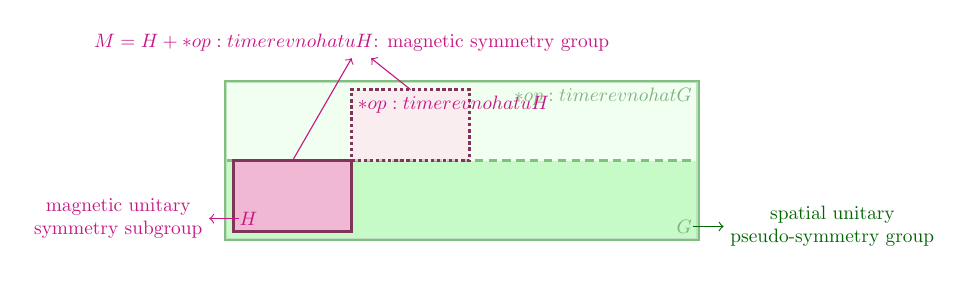
\begin{tikzpicture}
  \onslide<3->{
    \fill[fill=green!90!black, opacity=.8] (0, 0) -- (6, 0) -- (6, 1) -- (0, 1) -- cycle;
    \filldraw[fill=green!20, fill opacity=.6, draw=green!50!black, very thick] (0, 0) -- (6, 0) -- (6, 2) -- (0, 2) -- cycle;
    \draw[densely dashed, draw=green!50!black, thick] (0, 1) -- (6, 1);
    \node[anchor=south east, inner sep=3pt, scale=.7, DarkGreen] (G) at (6, 0) {$\symcal{G}$};
    \node[anchor=north east, inner sep=3pt, scale=.7, DarkGreen] at (6, 2) {$\gls*{op:timerevnohat} \symcal{G}$};
  }
  \onslide<8->{
    \filldraw[fill=white, draw=white, opacity=.5, very thick] (0, 0) -- (6, 0) -- (6, 2) -- (0, 2) -- cycle;
    \fill[fill=HotPink!90!black, opacity=.8] (0.1, 0.1) -- (1.6, 0.1) -- (1.6, 1) -- (0.1, 1) -- cycle;
    \filldraw[fill=HotPink!20, fill opacity=.6, draw=HotPink!50!black, very thick] (0.1, 0.1) -- (1.6, 0.1) -- (1.6, 1) -- (0.1, 1) -- cycle;
    \filldraw[fill=HotPink!20, fill opacity=.6, draw=HotPink!50!black, very thick, densely dotted] (1.6, 1) -- (3.1, 1) -- (3.1, 1.9) -- (1.6, 1.9) -- cycle;
    \node[anchor=south west, inner sep=3pt, scale=.7, MediumVioletRed] (H) at (0.1, 0.1) {$\symcal{H}$};
    \node[anchor=north west, inner sep=3pt, scale=.7, MediumVioletRed] at (1.6, 1.9) {$\gls*{op:timerevnohat} u \symcal{H}$};
  }
  \onslide<9->{
    \draw[->, DarkGreen, shorten <=-2] (G) -- ++(0.5, 0) node[scale=.7, anchor=west, align=center] {spatial unitary\\ pseudo-symmetry group};
    \draw[->, MediumVioletRed, shorten <=-2] (H) -- ++(-0.5, 0) node[scale=.7, anchor=east, align=center] {magnetic unitary\\ symmetry subgroup};
    \draw[->, MediumVioletRed] (0.85, 1) -- ++(0.75, 1.3) node[scale=.7, anchor=south, align=center] (maggroup) {$\symcal{M} = \symcal{H} + \gls*{op:timerevnohat} u \symcal{H}$: magnetic symmetry group};
    \draw[->, MediumVioletRed] (2.35, 1.9) -- (maggroup);
  }
\end{tikzpicture}